\section{Sistema BikeX}
\label{sec:sistema_bikex}

%Software Bikex: modelagem (uml), linguagem, signals, arquitetura
\subsection{Módulos}
Esta seção visa descrever como os diversos módulos do sistema irão se comportar separadamente e como vão interagir entre si. O sistema será composto pelos Unity, Bikex, Device. A figura \ref{diagrama-classes} exemplifica como os módulos interagem entre si.

O módulo Unity será responsável com as interações entre o usuário e o sistema. A primeira responsabilidade é retornar para o sistema a altitude atual do usuário. Essa informação será usada para definir se é necessário o acionamento da frenagem para simular uma inclinação no ambiente virtual. Outra responsabilidade será definir a posição e rotação atual do usuário no sistema. Essas informações irão ser disponibilizadas com a interação de outros módulos. Algumas informaçòes serão disponibilizadas pelo sistema para o usuário. Informações como: velocidade, distância e a velocidade máxima atingida pelo usuário. Por fim, esse módulo irá fazer a renderização do frame para o usuário. Essa renderização irá considerar todas as interações com o sistema e as informações geradas com essa interação.

\begin{figure}[h]
  \centering
	%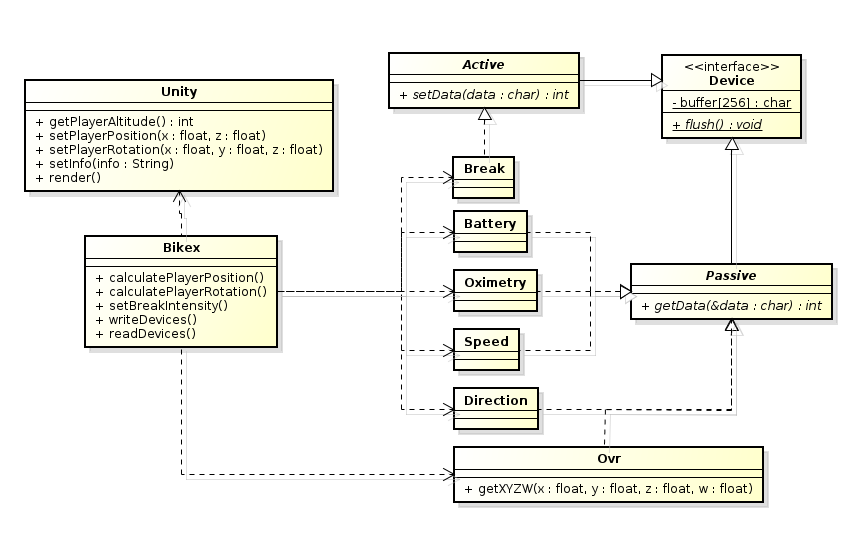
\includegraphics[scale=0.5]{figuras/diagrama_de_classe}
  \caption{Diagrama de classes}
  \label{diagrama-classes}
\end{figure}

No sistema terá um módulo que será composto por várias classes. Esse módulo, que é o responsável em fazer a interação com os dispositivos externos, se chama Device. Primeiramente, a classe principal será uma interface chamada Device. Duas classes irão relacionar com essa interface diretamente, a Active e a Passive. A classe Active representará os dispositivos que irão influenciar ativamente e fisicamente no sistema. Essa classe irá ser responsável por informar os dados para essa influência no sistema. Um dispositivo que exemplificar é a frenagem do sistema. A classe Passive são dispositivos que fornecem informações para o sistema. Os dispositivos de velocidade, direção e OVR são exemplos desse tipo de Device. A classe Passive irá ser responsável de coletar informações desses dispositivos e fornecer para o sistema realizar os procedimentos necessários. O dispositivo OVR é o Oculus em si e será responsável em fornecer a posição da cabeça do usuário.

O módulo Bikex é o módulo central do sistema e fará a interface com o módulo Unity e os outros módulos. Esse módulo é responsável por receber as informações dos dispositivos do tipo Passive e fazendo as transformações necessárias para enviar para o módulo Unity. O primeiro procedimento que esse módulo realiza é o cálculo da posição do usuário e tem como entrada a velocidade e a direção atuais do usuário. Outro procedimento será o cálculo da rotação do usuário. Isso será feito a partir de dados fornecidos pelo dispositivo Oculus. Essa rotação definirá a direção que o usuário está olhando. Definimos a separação desses dois procedimentos para que a rotação da cabeça do usuário não interfira na rotação da bicicleta. O outro procedimento é definir a intensidade de frenagem de acordo com a altitude coletada do módulo Unity. A partir dessa intensidade, o Bikex aciona o dispositivo de freio com a mesma.



%Unity: scripts, modelagem, assets etc
\subsection{Unity}

%Python: versao do python, modulos puppet, modulos para comunicacao UART
\subsection{Python}

%Falar aqui sobre o software do bikex, a integracao do python/msp430/unity
\subsection{Integração Sensores e Sistema}
